\documentclass{article}
\usepackage{amsmath}
\usepackage{array}
\usepackage{color}
\usepackage{graphicx}
\usepackage{float} % utiliser H pour forcer a mettre l'image ou on veut
\usepackage{lscape} % utilisation du mode paysage
\usepackage{mathbbol} % permet d'avoir le vrai symbol pour les reels grace a mathbb
\usepackage{enumerate} % permet d'utiliser enumerate
\usepackage{marvosym} % permet d'avoir le symbol pour le nucleaire
\usepackage{moreverb} % permet d'utiliser verbatimtab : conservation la tabulation
\usepackage{stmaryrd} % permet d'utiliser \llbrackedt et \rrbracket : double crochet
\usepackage{noabbrev]{cleveref} % permet d'utiliser cref and Cref


\setlength {\textwidth}{16.6cm}
\setlength {\textheight}{21cm}
\setlength {\oddsidemargin}{0cm}
\setlength{\headsep}{5pt} 

\newcommand\bn{\boldsymbol{\nabla}}
\newcommand\bo{\boldsymbol{\Omega}}
\newcommand\br{\mathbf{r}}
\newcommand\la{\left\langle}
\newcommand\ra{\right\rangle}
\newcommand\bs{\boldsymbol}
\newcommand\red{\textcolor{red}}
\newcommand\ldb{\{\!\!\{}
\newcommand\rdb{\}\!\!\}}
\newcommand\llb{\llbracket}
\newcommand\rrb{\rrbracket}

\renewcommand{\(}{\left(}
\renewcommand{\)}{\right)}
\renewcommand{\[}{\left[}
\renewcommand{\]}{\right]}


\begin{document}
\title{Tests}
\author{Bruno Turcksin} 
\date{}
\maketitle

\section{Adaptive Mesh Refinement test}
There are 10720 cells: 10482 quadrilaterals, 236 pentagons, and 2 hexagons 
for a total of 43120 degrees of freedom. The distribution is given by:
\begin{figure}[H]
  \centering
  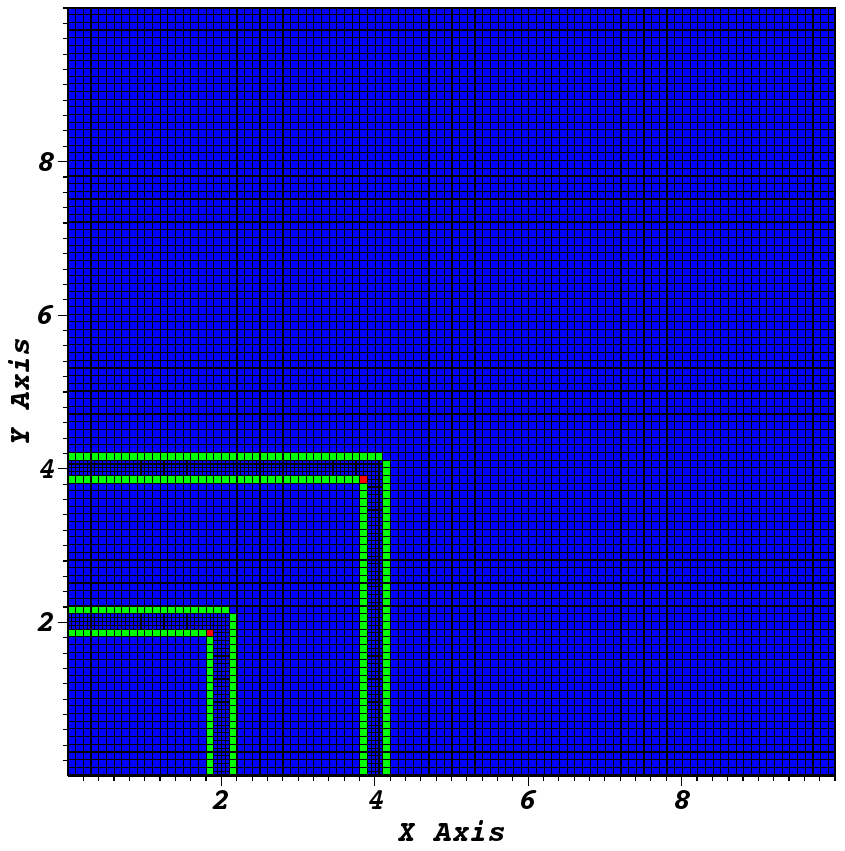
\includegraphics[width=4cm]{polygon_amr}
  \caption{Polygons distribution}
\end{figure}
\begin{itemize}
  \item Blue cells are quadrilaterals.
  \item Green cells are pentagons.
  \item Red cells are hexagons.
\end{itemize}
The domain is composed if three zones:
\begin{description}
  \item[Green zone:] $\Sigma_t=1cm^{-1}$, $\Sigma_s=0.9cm^{-1}$,
    source=$1cm^{-3}s^{-1}$
  \item[Red zone:] $\Sigma_t=1.5cm^{-1}$, $\Sigma_s=1.44cm^{-1}$, no source
  \item[Blue zone:] $\Sigma_t=1cm^{-1}$, $\Sigma_s=0.3cm^{-1}$, no source
\end{description}
We use a $S_{16}$ GLC quadrature, with SI, tolerance is $10^{-8}$, PWLD,
bottom and left boundaries are reflective, right and top boundaries vacuum.
\begin{table}[H]
  \caption{Comparison of preconditioners on AMR mesh.}
  \begin{centering}
    \begin{tabular}{|c|c|c|c|c|c|c|}
      \hline
       & No-DSA & CG & PCG-SGS & PCG-MLU & PCG-MLM & AGMG \\
      \hline
      SI iter    & 184     & 19      &
      Prec (s)   & NA      & NA      &
      MIP (s)    & NA      & 48.1908 &
      CG iter    & NA      & 11300   & 4734
      Total (s)  & 802.985 & 138.825 &
    \end{tabular}
  \end{centering}
\end{table}


\end{document}
